% AI-Intent: Conceptual Modeling for Accountable Multi-Agent AI Systems
% Springer LNCS format for ER 2026 (Conceptual Modeling Conference)

\documentclass[runningheads]{llncs}

\usepackage[T1]{fontenc}
\usepackage{graphicx}
\usepackage{booktabs}
\usepackage{amsmath}
\usepackage{amssymb}
\usepackage{listings}
\usepackage{xcolor}
\usepackage{hyperref}
\usepackage{tikz}
\usetikzlibrary{arrows.meta, positioning, shapes.geometric, fit}

\lstset{
  basicstyle=\ttfamily\small,
  keywordstyle=\color{blue}\bfseries,
  stringstyle=\color{red!70!black},
  commentstyle=\color{green!50!black}\itshape,
  breaklines=true,
  frame=single,
  numbers=left,
  numberstyle=\tiny\color{gray},
  backgroundcolor=\color{gray!5},
  captionpos=b,
  aboveskip=8pt,
  belowskip=8pt,
}

\begin{document}

\title{AI-Intent: A Conceptual Modeling Framework\\
for Accountable Multi-Agent AI Systems}

\author{Wolfgang Maa\ss\inst{1} \and Iris Reinhartz-Berger\inst{2}}

\authorrunning{W.~Maa\ss{} and I.~Reinhartz-Berger}

\institute{German Research Center for Artificial Intelligence (DFKI)\\
and Saarland University, Saarbr\"ucken, Germany\\
\email{wolfgang.maass@dfki.de}
\and University of Haifa, Haifa, Israel\\
\email{iris@is.haifa.ac.il}}

\maketitle

\begin{abstract}
Existing agent-oriented conceptual modeling frameworks were designed for
components with deterministic semantics. When applied to large language
model (LLM)-based agents---whose behavior is stochastic, emergent, and
shaped by natural-language mandates---these frameworks lack three
constructs that governance and accountability require: a representation
of the \emph{boundary of legitimate action} (distinct from goal
satisfaction), \emph{negative obligations} enforceable at runtime, and
a \emph{communication-as-evidence} layer that makes every inter-agent
message an auditable artifact. We introduce \textsc{AI-Intent}, a
conceptual modeling framework that supplies these constructs through
three first-class modeling artifacts: the \emph{Agent Manifest}
(declaring intent scope, boundary constraints, and risk parameters),
the \emph{Compliance Agent} (a mandatory gatekeeper that enforces
manifests before message delivery), and the \emph{Accountability Trace}
(a derived session artifact recording what was decided and what was
prevented). We ground the framework in a metamodel with explicit
ontological commitments, relate it formally to deontic logic and
existing agent-oriented frameworks, and validate it through a reference
implementation for private investment advisory. A 190-evaluation
empirical study (10 independent runs, 19 test cases, four adversarial
disposition presets) shows boundary violation containment averaging
97.9\% across all runs. We argue that the compliance agent is not an
engineering convenience but a structural modeling necessity: in the
reference implementation, the materials agent violated its allocation cap
on first attempt in 12.9\% of neutral-disposition sessions, motivating
external enforcement as a required component in any governance-oriented
conceptual model for multi-agent AI systems.

\keywords{Multi-Agent Systems \and Conceptual Modeling \and LLM
Agents \and Accountability \and Agent Manifests \and Deontic Logic
\and Normative Systems \and Governance}
\end{abstract}

%=====================================================================
\section{Introduction}
\label{sec:introduction}
%=====================================================================

Large language model (LLM)-based agents are rapidly moving from research
prototypes to production systems that make consequential decisions in
finance, healthcare, and enterprise
operations~\cite{wang2024survey,xi2023rise}. Unlike traditional software
components whose behavior is fully determined by source code, LLM agents
exhibit \emph{emergent} behavior shaped by prompts, training data, and
stochastic decoding. When multiple such agents collaborate---delegating
subtasks, synthesizing partial results, and producing joint
recommendations---the resulting system raises questions that existing
conceptual models are not equipped to answer: \emph{what} was each agent
supposed to do, \emph{whether} it stayed within its designated scope, and
\emph{why} a particular output was produced.

Conceptual modeling frameworks for multi-agent systems have a rich
history~\cite{yu2011social,bresciani2004tropos,wooldridge2000gaia}.
They model agents in terms of goals, capabilities, roles, and
inter-agent dependencies, providing formal foundations for requirements
analysis and system design. However, they share an assumption that their
target components have deterministic or rule-governed semantics. This
assumption does not hold for LLM agents. Three modeling gaps result:

\textbf{Gap 1 — Intent boundary vs.\ goal satisfaction.} Traditional
goal models (e.g., $i^*$, Tropos) treat goal satisfaction as
graded~\cite{yu2011social}: softgoals can be partially achieved,
contributing positively or negatively to parent goals. For LLM agents,
the relevant construct is not graded goal satisfaction but a binary
\emph{intent boundary}: a request either falls within the agent's
legitimate mandate or it does not. An equity analyst agent recommending
gold at 35\% allocation has not partially satisfied its goal; it has
violated its mandate scope. Existing frameworks have no construct for
this boundary.

\textbf{Gap 2 — Negative obligations as runtime-enforceable constraints.}
Normative frameworks and deontic logic provide well-developed accounts
of obligation, permission, and
prohibition~\cite{vonwright1951essay,governatori2005meeting,
boella2006introduction}. In classical normative agent architectures,
norms are represented declaratively and reasoned about by the agent
itself~\cite{dignum1999autonomous}. For LLM agents, self-reasoning over
norms is unreliable: stochastic generation means agents may acknowledge
a constraint and then violate it, or construct plausible arguments for
exceptions. The modeling challenge is to represent negative obligations
in a form that an \emph{external} enforcement component can evaluate,
not one that relies on agent self-compliance.

\textbf{Gap 3 — Communication as audit evidence.} Existing agent
communication models (e.g., FIPA-ACL~\cite{fipa2002}) specify message
syntax and semantics but treat communication logs as an optional
engineering concern. Regulatory frameworks for AI systems (EU AI
Act~\cite{euaiact2024}, MiFID II in finance) require that every
consequential decision be traceable to its inputs. This requires
communication logging as a \emph{structural property} of the
metamodel, not an add-on.

We propose \textsc{AI-Intent}, a conceptual modeling framework that
addresses all three gaps. Its contributions are:

\begin{enumerate}
    \item A \textbf{metamodel} with explicit ontological commitments that
    introduces intent scope, boundary constraints, and risk parameters as
    first-class modeling constructs, formally related to deontic concepts
    of prohibition and obligation.

    \item The \textbf{Agent Manifest} as an operative modeling artifact:
    simultaneously a specification, a normative contract, and a runtime
    enforcement document injected as the LLM system prompt.

    \item The \textbf{Compliance Agent} as a required structural
    component in the metamodel: a mandatory gatekeeper that enforces
    manifests before message delivery, grounded in the empirical finding
    that LLM agent self-compliance is insufficient.

    \item The \textbf{Accountability Trace} as a derived session artifact
    that records not only what was decided but what was prevented,
    satisfying both machine-processable and human-readable audit
    requirements.

    \item A \textbf{comparative analysis} against existing frameworks
    ($i^*$, Tropos, GAIA, NMAS, MCP) showing which governance scenarios
    each can and cannot model.

    \item A \textbf{reference implementation} in a private investment
    advisory domain, validated through 190 evaluations with adversarial
    agent disposition presets.
\end{enumerate}

%=====================================================================
\section{Background and Related Work}
\label{sec:background}
%=====================================================================

\subsection{Agent-Oriented Conceptual Modeling}

Agent-oriented modeling frameworks provide the foundation this work
extends. We review the most relevant and identify their limitations for
the LLM agent setting.

\textbf{The $i^*$ framework}~\cite{yu2011social} models actors with
goals, tasks, resources, and softgoals connected by contribution links.
Its softgoal construct explicitly models partial satisfaction: a design
decision may \emph{make}, \emph{help}, \emph{hurt}, or \emph{break} a
softgoal, enabling nuanced trade-off analysis. This graded satisfaction
is appropriate for modeled agent preferences but is the wrong construct
for mandate boundaries. Whether a stocks agent recommends gold (clearly
outside mandate) or recommends a 10.5\% position (marginally outside the
10\% limit) are categorically different from the perspective of
constraint enforcement: both are violations, neither is a partial
achievement.

\textbf{Tropos}~\cite{bresciani2004tropos} extends $i^*$ into a
full software development methodology covering early and late
requirements, architectural design, and detailed design. Tropos
introduces ``plans'' as sequences of activities satisfying goals, and
capability models linking agents to the plans they can execute. The
framework has no construct for prohibitions: it models what agents can
and should do, not what they must not do.

\textbf{GAIA}~\cite{wooldridge2000gaia} provides role models (with
permissions, responsibilities, activities, and protocols) and interaction
models. GAIA's permission construct is the closest existing analog to
boundary constraints: a role's permissions define the actions it is
allowed to take. However, GAIA permissions are granted by system
designers at modeling time and assumed to hold at runtime; there is no
mechanism for runtime verification that an agent operating in a role
stays within its permissions. For deterministic agents this assumption
is safe; for stochastic LLM agents it is not.

\textbf{Normative Multi-Agent Systems (NMAS)} address obligation and
prohibition more directly~\cite{boella2006introduction,
governatori2005meeting,dignum1999autonomous}. Norm-governed agent
architectures represent norms as explicit objects that agents reason
about, with deontic operators for obligation ($\mathbf{O}$), permission
($\mathbf{P}$), and prohibition ($\mathbf{F}$)~\cite{vonwright1951essay}.
Governatori et al.'s defeasible deontic
logic~\cite{governatori2005meeting} allows norms to have exceptions and
to be defeated by stronger norms, which is appropriate for complex
multi-stakeholder settings. However, these approaches assume agents that
\emph{deliberate} over norms: they evaluate their intended actions
against applicable norms before acting. LLM agents do not deliberate in
this sense; they generate text that may or may not comply with norms
depending on how those norms are represented in the prompt and how
reliably the model follows instructions. This motivates our approach of
externalizing norm enforcement to a dedicated compliance component
rather than relying on agent norm-reasoning.

\subsection{Model-Driven Approaches and Operative Models}

The AI-Intent manifest-to-prompt transformation is an instance of
model-to-text (M2T) transformation in model-driven engineering
(MDE)~\cite{brambilla2012model}. In MDE, M2T transformations generate
artifacts (code, configuration, documentation) from platform-independent
models. The distinctive feature of AI-Intent's M2T transformation is that
the generated artifact is a \emph{natural-language system prompt} that
shapes the behavior of a stochastic generative model. This blurs the
traditional MDE distinction between model and code: the manifest is
simultaneously a conceptual model (expressing intent and constraints at
an abstract level) and an operative specification (directly executed by
the LLM). We term this property \emph{model operativity} and argue it is
a characteristic feature of conceptual models for AI systems.

\subsection{AI Governance and Accountability}

The EU AI Act~\cite{euaiact2024} classifies AI systems by risk tier and
mandates transparency, auditability, and human oversight for high-risk
applications. Financial AI systems are subject to additional requirements
under MiFID II, requiring that investment recommendations be traceable to
their inputs and that conflicts of interest be disclosed. Existing
accountability frameworks address individual model
decisions~\cite{arrieta2020explainable} and dataset
documentation~\cite{gebru2021datasheets,mitchell2019model}, but not
\emph{multi-agent accountability}: the challenge of tracing a decision
produced by multiple collaborating AI components. AI-Intent addresses
this through the accountability trace as a structural artifact of the
communication model. Enterprise architecture standards and SOA compliance
logging provide audit trails as infrastructure services, but these treat
the audit log as an operational artifact external to the system model: it
records what happened but is not a first-class element of the metamodel
that constrains system behavior. In AI-Intent, the accountability trace
is a structural model component: its existence is a well-formedness
condition, and the compliance verdict attached to each message is a
metamodel relationship, not a log entry. This distinction---between
logging as infrastructure and communication-as-evidence as a metamodel
property---is the modeling gap we address.

\subsection{Multi-Agent LLM Architectures}

AutoGen~\cite{wu2023autogen}, CrewAI~\cite{crewai2024}, and
LangGraph~\cite{langgraph2024} enable LLM agents to collaborate through
role assignment, tool use, and conversational orchestration. These
frameworks represent agent roles as free-text strings with no formal
semantics, no runtime constraint verification, and no audit trail. The
Model Context Protocol (MCP)~\cite{anthropic2024mcp} standardizes
LLM-to-tool communication through a client-server architecture, providing
interoperability but not governance. AI-Intent builds on MCP's
communication substrate and adds the governance layer it lacks.

LLM guardrail systems such as NeMo
Guardrails~\cite{rebedea2023nemo} and Constitutional
AI~\cite{bai2022constitutional} address output safety for individual
models through input/output filtering and self-critique. These systems
enforce constraints on single-agent outputs but do not model inter-agent
accountability: they cannot trace a multi-agent decision to its
constituent sub-agent outputs, do not maintain compliance histories
across revision cycles, and do not produce structured audit artifacts.
AI-Intent's compliance agent shares the guardrails motivation (constraint
enforcement on stochastic outputs) but operates at the multi-agent
communication level rather than the single-model output level.

%=====================================================================
\section{The AI-Intent Framework}
\label{sec:framework}
%=====================================================================

\subsection{Core Principles and Ontological Commitments}
\label{sec:ontology}

AI-Intent adopts the following ontological commitments, grounded in
the Unified Foundational Ontology (UFO)~\cite{guizzardi2005ontological}
and standard deontic
semantics~\cite{vonwright1951essay,governatori2005meeting}:

\begin{description}
    \item[Agents as intentional objects.] Following UFO, we treat agents
    as \emph{intentional objects} with dispositions to act in certain
    ways~\cite{guizzardi2005ontological}. An agent's manifest specifies
    the \emph{intended disposition}: the range of behaviors the agent is
    designed to exhibit.

    \item[Intent scope as a sortal boundary.] The intent scope is not a
    goal (which admits degrees of satisfaction) but a \emph{sortal
    boundary}: it defines the category of situations to which the agent's
    competence applies. Formally, the scope induces a partition of the
    query space into \emph{in-scope} and \emph{out-of-scope} regions.
    This is a binary, not graded, distinction.

    \item[Boundary constraints as prohibitions.] Following deontic
    logic~\cite{vonwright1951essay}, boundary constraints are
    \emph{prohibitions} of the form $\mathbf{F}(\phi)$: the agent is
    forbidden from producing outputs satisfying predicate $\phi$. Risk
    parameters provide the quantitative instantiations: $\mathbf{F}
    (\mathit{allocation} > 0.15)$ for a 15\% cap. Unlike NMAS norms,
    these prohibitions are not reasoned about by the agent but enforced
    by an external compliance component.

    \item[Compliance as a structural role.] The compliance agent is not
    an optional add-on but a \emph{structural role} in the metamodel: the
    role that makes prohibitions operative. A framework without a
    compliance role can represent prohibitions but cannot enforce them. We
    argue this structural necessity follows from the empirical finding
    that LLM agent self-compliance is insufficient (Section~\ref
    {sec:compliance}).

    \item[Communication as evidence.] Every inter-agent message is an
    \emph{event} in the UFO sense: a particular, time-stamped occurrence
    that cannot be repeated or undone. The MCP message log is an ordered
    set of such events constituting a complete history of the session.
    The accountability trace is a \emph{situation}---a structured
    snapshot of relevant aspects of that history---derived from the event
    log.
\end{description}

\subsection{Metamodel}
\label{sec:metamodel}

Figure~\ref{fig:metamodel} presents the AI-Intent metamodel. We describe
each construct with its ontological type, multiplicity constraints, and
well-formedness conditions.

\begin{figure}[t]
\centering
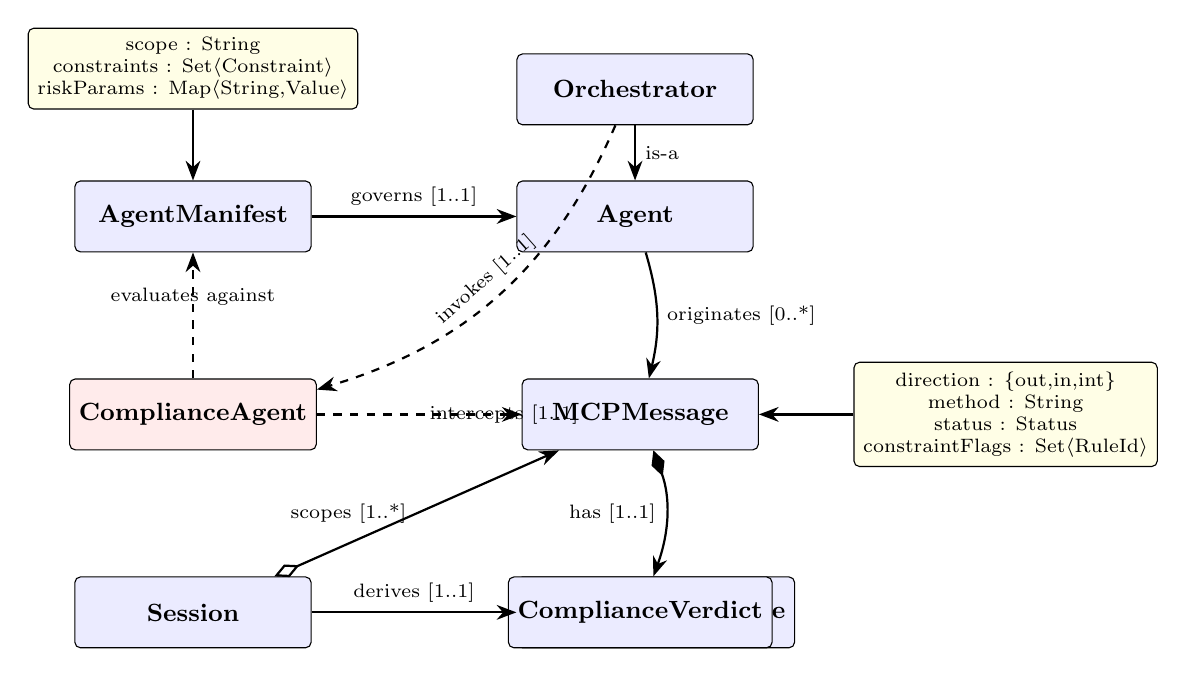
\begin{tikzpicture}[
    node distance=1.5cm and 2.4cm,
    every node/.style={font=\small},
    class/.style={rectangle, draw, fill=blue!8, minimum width=3.0cm,
        minimum height=0.9cm, align=center, rounded corners=2pt},
    normclass/.style={rectangle, draw, fill=red!8, minimum width=3.0cm,
        minimum height=0.9cm, align=center, rounded corners=2pt},
    attr/.style={rectangle, draw, fill=yellow!10, minimum width=2.8cm,
        minimum height=0.7cm, align=center, font=\scriptsize,
        rounded corners=2pt},
    rel/.style={-{Stealth[length=2.5mm]}, thick},
    comp/.style={{Diamond[open, length=3.5mm]}-{Stealth[length=2.5mm]}, thick},
    fcomp/.style={{Diamond[length=3.5mm, fill=black]}-{Stealth[length=2.5mm]}, thick},
    dep/.style={-{Stealth[length=2.5mm]}, thick, dashed},
]

\node[class] (manifest) {\textbf{AgentManifest}};
\node[class, right=2.6cm of manifest] (agent) {\textbf{Agent}};
\node[class, above=0.7cm of agent] (orch) {\textbf{Orchestrator}};
\node[normclass, below=1.6cm of manifest] (compliance)
    {\textbf{ComplianceAgent}};
\node[class, right=2.6cm of compliance] (message) {\textbf{MCPMessage}};
\node[class, below=1.6cm of compliance] (session) {\textbf{Session}};
\node[class, right=2.6cm of session] (trace)
    {\textbf{AccountabilityTrace}};
\node[class, below=1.6cm of message] (verdict)
    {\textbf{ComplianceVerdict}};

\node[attr, above=0.9cm of manifest] (mattr)
    {scope : String\\
     constraints : Set$\langle$Constraint$\rangle$\\
     riskParams : Map$\langle$String,Value$\rangle$};

\node[attr, right=1.2cm of message] (msgattr)
    {direction : $\{$out,in,int$\}$\\
     method : String\\
     status : Status\\
     constraintFlags : Set$\langle$RuleId$\rangle$};

% Multiplicities and relationships
\draw[rel] (manifest) --
    node[above, font=\scriptsize] {governs [1..1]}
    (agent);
\draw[dep] (compliance) --
    node[above, font=\scriptsize] {evaluates against}
    (manifest);
\draw[rel] (agent) to[bend left=15]
    node[right, font=\scriptsize] {originates [0..*]}
    (message);
\draw[dep] (compliance) --
    node[right, font=\scriptsize] {intercepts [1..1]}
    (message);
\draw[comp] (session) --
    node[left, font=\scriptsize] {scopes [1..*]}
    (message);
\draw[rel] (session) --
    node[above, font=\scriptsize] {derives [1..1]}
    (trace);
\draw[fcomp] (message) to[bend left=20]
    node[left, font=\scriptsize] {has [1..1]}
    (verdict);
\draw[rel] (orch) -- node[right, font=\scriptsize] {is-a} (agent);
\draw[dep] (orch) to[bend left=25]
    node[above, font=\scriptsize, sloped] {invokes [1..1]}
    (compliance);
\draw[rel] (mattr) -- (manifest);
\draw[rel] (msgattr) -- (message);

\end{tikzpicture}
\caption{AI-Intent metamodel. Solid diamonds denote composition;
open diamonds aggregation; dashed arrows dependency.
\texttt{ComplianceAgent} (shaded) is a structural role, not an optional
component: every \texttt{MCPMessage} has exactly one associated
\texttt{ComplianceVerdict} (composition). The \texttt{Orchestrator}
specializes \texttt{Agent} and invokes the \texttt{ComplianceAgent}
for every message. \texttt{AccountabilityTrace}
is derived from \texttt{Session}.}
\label{fig:metamodel}
\end{figure}

\textbf{Well-formedness conditions:}
\begin{enumerate}
    \item Every \texttt{Agent} is governed by exactly one
    \texttt{AgentManifest}: $\forall a \in \mathtt{Agent}: |\{m \in
    \mathtt{Manifest} \mid m.\mathit{governs} = a\}| = 1$
    \item Every \texttt{MCPMessage} has exactly one
    \texttt{ComplianceVerdict}: no message is delivered without
    compliance evaluation.
    \item Every \texttt{Session} derives exactly one
    \texttt{AccountabilityTrace}.
    \item \texttt{AgentManifest} instances are immutable: $\forall m:
    \nexists$ update operation on $m$ after instantiation.
    \item The \texttt{constraints} set of a manifest is non-empty:
    $\forall m: |m.\mathit{constraints}| \geq 1$
    \item Every \texttt{Session} has exactly one \texttt{Orchestrator}
    instance: $\forall s \in \mathtt{Session}: |\{o \in
    \mathtt{Orchestrator} \mid o \in s\}| = 1$.
\end{enumerate}

\subsection{Agent Manifest}
\label{sec:manifest}

The \texttt{AgentManifest} is a \emph{type-level} artifact: it defines
the behavioral type of an agent, in the same sense that a class defines
the type of its instances in object-oriented modeling. Unlike a class,
whose methods have fixed implementations, a manifest's constraints are
evaluated at runtime against stochastically generated outputs.

Formally, a manifest $M$ is:
\begin{equation}
M = \langle \mathit{id}, \mathit{name}, \mathit{role},
    \mathit{scope}, C, R, \mathit{summary} \rangle
\end{equation}

\noindent where $\mathit{scope} \in \mathcal{L}$ is a natural-language
statement defining the agent's sortal boundary (Section~\ref{sec:ontology}),
$C = \{c_1, \ldots, c_n\}$ is a finite set of \emph{constraints}, each
a pair $c_i = \langle \mathit{text}_i, \phi_i \rangle$ with natural-language
statement $\mathit{text}_i$ and machine-evaluable predicate $\phi_i$, and
$R: \mathit{Name} \rightarrow \mathit{Value}$ maps risk parameter names
to their bounds.

The distinction between $\mathit{scope}$ and $C$ corresponds to the
deontic distinction between \emph{competence} and \emph{prohibition}:
$\mathit{scope}$ defines what the agent is competent to address;
$C$ defines what the agent is forbidden from producing, independent
of whether the request is in-scope. A materials agent is competent to
advise on gold (in-scope) but forbidden from recommending more than 15\%
allocation (boundary constraint). Both must be represented and enforced.

\subsubsection{Manifest Operativity.}

A manifest $M$ is transformed into an LLM system prompt via a
deterministic function $\mathit{prompt}: M \rightarrow \mathcal{L}$. The
transformation produces a structured natural-language document that
includes the intent scope, all constraint texts, and all risk parameter
values, followed by a meta-constraint:

\begin{quote}
\itshape ``If a request falls outside your intent scope or violates any
boundary constraint, you must explicitly identify the violated constraint
and decline. Do not silently comply with out-of-scope requests.''
\end{quote}

This property --- that the conceptual model is simultaneously a design
artifact and a runtime enforcement document --- we term \emph{model
operativity}. It distinguishes AI-Intent manifests from Model
Cards~\cite{mitchell2019model} and Datasheets~\cite{gebru2021datasheets},
which are documentation artifacts with no operative effect on the
described system's behavior.

\subsection{Compliance Agent}
\label{sec:compliance}

The \textbf{Compliance Agent} is the structural component that makes
boundary constraints operative. As established in Section~\ref{sec:ontology},
prohibitions require an enforcement component that can evaluate them
externally to the constrained agent. The compliance agent fills this role.

\subsubsection{Necessity Argument.}

We claim the compliance agent is a structural necessity, not an
engineering option. This claim rests on the following argument:

\begin{enumerate}
    \item LLM agents are stochastic: identical prompts may produce
    different outputs on different invocations.
    \item Boundary constraints are prohibitions that must hold on every
    invocation, not on average across invocations.
    \item Ensuring (2) for (1) requires evaluation of each output
    individually before any consequential action (delivery) is taken.
    \item The agent whose output is being evaluated cannot be the
    evaluator: self-evaluation is subject to the same stochasticity as
    the original output~\cite{huang2023selfcorrect}.
    \item Therefore, constraint enforcement requires a component external
    to the constrained agent that evaluates each output before delivery.
\end{enumerate}

This argument is supported empirically: across the 129 sessions in which
the materials agent was consulted (out of 190 total evaluations with four
disposition presets), it violated its 15\% allocation cap on first attempt
in 25.6\% of cases. Crucially, under the neutral disposition preset---in
which agents had no adversarial modification---the first-attempt violation
rate was 12.9\% (13 of 101 neutral sessions). Under adversarial presets
(\textit{aggressive\_broker}, \textit{reckless\_portfolio}), the rate
rose to 100\%. Self-compliance is insufficient under any disposition.

\subsubsection{Formal Specification.}

For each intercepted message, the compliance agent produces a verdict:

\begin{equation}
V = \langle \mathit{approved}, \mathit{violations},
    \mathit{ruleIds}, \mathit{basis}, \mathit{instruction},
    \mathit{msgId} \rangle
\end{equation}

\noindent where $\mathit{approved} \in \{\top, \bot\}$,
$\mathit{violations} \subseteq \mathit{String}$ lists rejection reasons,
$\mathit{ruleIds} \subseteq \mathit{RuleId}$ identifies the violated
constraints from the sender's manifest, $\mathit{basis}$ cites the
regulatory or manifest source, and $\mathit{instruction}$ provides the
revision directive when $\mathit{approved} = \bot$.

Constraint evaluation proceeds in two layers, with a precedence rule:

\textbf{Deterministic evaluation} ($\mathit{eval}_D$) applies
machine-computable predicates to structured output fields: numerical
comparisons against risk parameters, substring detection for prohibited
terms, credit rating classification, maturity bucket aggregation. These
checks are reproducible and model-independent.

\textbf{Semantic evaluation} ($\mathit{eval}_S$) applies an LLM to rules
whose predicates cannot be expressed in closed form over structured
fields (e.g., ``must provide inflation correlation rationale'').

\textbf{Precedence rule:} $\forall$ rule $r$: if
$\mathit{eval}_D(r) = \mathit{pass}$ then the compliance verdict for $r$
is $\mathit{pass}$, regardless of $\mathit{eval}_S(r)$. Semantic checks
apply only where deterministic evaluation is inapplicable. This prevents
LLM-based semantic evaluation from overriding deterministic constraint
satisfaction.

\subsubsection{Revision Protocol and Termination.}

When $\mathit{approved} = \bot$, the compliance agent initiates a
revision cycle. Let $\mathit{maxRev} \in \mathbb{N}$ be the maximum
revision count (default: 2, scaled by disposition preset).

\begin{definition}[Compliance Protocol]
For a message $\mu$ from agent $a$ to agent $b$:
\begin{enumerate}
    \item Compute $V = \mathit{evaluate}(\mu, M_a)$.
    \item If $V.\mathit{approved} = \top$: deliver $\mu$ to $b$;
    log $V$ as \texttt{compliance.approve}.
    \item If $V.\mathit{approved} = \bot$ and revision count
    $< \mathit{maxRev}$: return $V.\mathit{instruction}$ to $a$;
    increment revision count; go to (1) with revised $\mu'$.
    \item If $V.\mathit{approved} = \bot$ and revision count
    $= \mathit{maxRev}$: issue $\mathit{forced\_block}$; log with
    $V.\mathit{ruleIds}$; do not deliver.
\end{enumerate}
\end{definition}

\textbf{Termination:} The protocol terminates in at most $\mathit{maxRev}
+ 1$ evaluations per message, since step (4) terminates unconditionally
at the bound. No infinite revision loop is possible.

\textbf{Safety:} No message with $\mathit{approved} = \bot$ is ever
delivered. This is enforced structurally: delivery is only possible
through step (2), which requires $\mathit{approved} = \top$.
$\mathit{forced\_pass}$ (delivering a rejected message) has no
corresponding operation in the protocol and cannot occur.

\textbf{Liveness (conditional):} If agent $a$ produces a response $\mu$
such that $\mathit{eval}_D(\mu) = \mathit{pass}$ for all applicable
rules, then $\mu$ is delivered in step (2) without revision. Liveness is
\emph{conditional} on the agent's ability to produce a compliant
response: the protocol guarantees delivery for compliant messages but
intentionally does not guarantee delivery for messages that remain
non-compliant after $\mathit{maxRev}$ revisions. This is a deliberate
design property of the protocol, not an LLM limitation.

\subsection{MCP Message Model}
\label{sec:mcp}

Every inter-agent communication is captured as:
\begin{equation}
\mu = \langle \mathit{id}, \mathit{sid}, t, d, \mathit{from},
    \mathit{to}, m, p, s, F, V \rangle
\end{equation}

\noindent where $d \in \{\mathit{outbound}, \mathit{inbound},
\mathit{internal}\}$, $m$ is the method identifier,
$p$ is the structured payload, $s \in S_{\mathit{status}}$ is the
response status with $S_{\mathit{status}} = \{\mathit{pending},
\mathit{ok}, \mathit{error}, \mathit{constraint\_violation},
\mathit{approved}, \mathit{forced\_block}\}$, $F \subseteq
\bigcup_{a} C_{M_a}$ is the set of constraint identifiers flagged, and
$V$ is the associated compliance verdict.

The status $\mathit{forced\_block}$ is terminal: no subsequent message
in the session may be sent from the blocked agent to any agent on the
same topic. This is enforced by the orchestrator: blocked agents are
excluded from synthesis.

\subsection{Orchestration Protocol}
\label{sec:orchestration}

The AI-Intent orchestration protocol has six steps:

\begin{enumerate}
    \item \textbf{Disposition activation:} Agent disposition scores are
    computed and logged as the first internal message, establishing the
    behavioral context for the session.
    \item \textbf{Query ingestion:} The user query $q$ is logged as
    $\mu_q = \langle \ldots, \mathit{user}, \mathit{central},
    \mathit{user.query}, q, \mathit{ok}, \emptyset, \top \rangle$.
    \item \textbf{Intent routing:} The orchestrator generates a routing
    plan $\rho = \langle A', Q' \rangle$ where $A' \subseteq A$ is the
    set of sub-agents to consult and $Q': A' \rightarrow \mathcal{L}$
    maps each to a sub-question. The routing plan is submitted to the
    compliance agent before any sub-agent is invoked.
    \item \textbf{Compliant parallel delegation:} For each $a \in A'$
    with approved routing, $Q'(a)$ is dispatched concurrently. Each
    invocation generates an outbound message, a compliance verdict, and
    (if approved) an inbound result.
    \item \textbf{Synthesis:} The orchestrator aggregates approved
    sub-agent results into a recommendation $r$ with an accountability
    note $\nu$. The synthesis message is submitted to the compliance agent
    before delivery.
    \item \textbf{Response delivery:} If the synthesis is approved, the
    final message $\mu_r$ is logged and delivered to the user.
\end{enumerate}

This protocol guarantees a minimum of $3n + 6$ MCP messages per session,
where $n = |A'|$ is the number of approved sub-agents consulted:
1 disposition + 1 query + 1 routing + 1 routing verdict + $2n$ agent
calls + $n$ analysis verdicts + 1 synthesis + 1 synthesis verdict +
1 response.

\subsection{Accountability Trace}
\label{sec:trace}

The \texttt{AccountabilityTrace} is a \emph{situation} (in the UFO
sense) derived from a complete session: a structured representation of
relevant aspects of the event history.

\begin{equation}
\mathit{trace}(\mathit{sid}) = \langle \mathit{sid}, t_{\mathit{gen}},
    q, A', \rho, \mathit{CC}, \mathit{CH}, B, n_\mu, r, L \rangle
\end{equation}

\noindent where $A'$ is the set of agents consulted, $\rho$ is the
routing rationale, $\mathit{CC}$ is the per-agent constraint check list,
$\mathit{CH}$ is the \emph{compliance history} (per-agent revision counts
and violated rule identifiers), $B$ is the set of permanently blocked
agents with block reasons and rule identifiers, $n_\mu$ is the total
message count, $r$ is the final recommendation, and $L$ is the ordered
message log.

The inclusion of $\mathit{CH}$ and $B$ is what distinguishes an
accountability trace from an audit log. An audit log records what
happened. An accountability trace records what happened and
\emph{what was prevented}, providing regulators with evidence of
both compliance and enforcement.

%=====================================================================
\section{Comparative Analysis}
\label{sec:comparison}
%=====================================================================

Table~\ref{tab:comparison} compares AI-Intent against the most relevant
existing frameworks across the modeling constructs required for LLM
agent governance. We consider three representative governance scenarios:

\textbf{S1 — Out-of-scope declination:} Agent must refuse a request
outside its mandate and name the constraint violated.

\textbf{S2 — Quantitative constraint enforcement:} Agent must not exceed
a numeric threshold (e.g., 15\% allocation cap); violations must be
detected and blocked.

\textbf{S3 — Cross-agent audit reconstruction:} An auditor must
reconstruct the full decision sequence from a session, including which
agents were consulted, which constraints fired, and what was blocked.

\begin{table}[t]
\centering
\caption{Comparative analysis of agent governance modeling capabilities.
\checkmark = fully expressible; $\circ$ = partially expressible with
significant extensions; $\times$ = not expressible without framework
revision.}
\label{tab:comparison}
\begin{tabular}{@{}lcccccc@{}}
\toprule
\textbf{Capability} & \textbf{$i^*$} & \textbf{Tropos} &
\textbf{GAIA} & \textbf{NMAS} & \textbf{MCP} &
\textbf{AI-Intent} \\
\midrule
Intent scope (binary mandate boundary) & $\times$ & $\times$ & $\circ$
    & $\circ$ & $\times$ & \checkmark \\
Negative obligations (prohibitions) & $\times$ & $\times$ & $\circ$
    & \checkmark & $\times$ & \checkmark \\
Quantitative risk parameters & $\times$ & $\times$ & $\times$
    & $\circ$ & $\times$ & \checkmark \\
Runtime constraint enforcement & $\times$ & $\times$ & $\times$
    & $\circ$ & $\times$ & \checkmark \\
External compliance gatekeeper & $\times$ & $\times$ & $\times$
    & $\times$ & $\times$ & \checkmark \\
Audit-native communication & $\times$ & $\times$ & $\times$
    & $\times$ & $\circ$ & \checkmark \\
Compliance history in trace & $\times$ & $\times$ & $\times$
    & $\times$ & $\times$ & \checkmark \\
Model operativity (runtime injection) & $\times$ & $\times$ & $\times$
    & $\times$ & $\times$ & \checkmark \\
\midrule
\textbf{S1 — Out-of-scope declination} & $\times$ & $\times$ & $\circ$
    & $\circ$ & $\times$ & \checkmark \\
\textbf{S2 — Quantitative enforcement} & $\times$ & $\times$ & $\times$
    & $\circ$ & $\times$ & \checkmark \\
\textbf{S3 — Audit reconstruction} & $\times$ & $\times$ & $\times$
    & $\times$ & $\circ$ & \checkmark \\
\bottomrule
\end{tabular}
\end{table}

\textbf{Notes on partial capabilities.} GAIA's permission construct
can represent that a role is not permitted to take certain actions, but
provides no runtime mechanism for verification. NMAS frameworks can
express prohibitions using deontic operators and reason about norm
violations, but the reasoning is performed by the agent being governed;
external enforcement is outside the NMAS modeling scope. MCP provides a
structured communication substrate that could, in principle, be extended
with audit logging, but this extension is not part of the specification.

We exclude guardrail systems (NeMo Guardrails, Constitutional AI) from
the table as they operate at the single-model output level rather than
the multi-agent communication level; Section~\ref{sec:background}
addresses their relationship to AI-Intent narratively.

The key differentiator of AI-Intent is not the representation of
individual constructs---NMAS handles prohibitions well, and GAIA handles
permissions---but their combination with runtime enforcement and model
operativity. An NMAS norm representation of ``allocation must not exceed
15\%'' is formally equivalent to AI-Intent's corresponding boundary
constraint, but the NMAS norm relies on agent self-compliance while
AI-Intent's compliance agent enforces it externally.

%=====================================================================
\section{Reference Implementation}
\label{sec:implementation}
%=====================================================================

We implemented AI-Intent as a Streamlit web application for private
investment advisory. The domain exhibits the characteristics that motivate
the framework: multiple specialized agents, clear regulatory requirements
(MiFID II), consequential decisions, and the need for auditable traces.

\subsection{Domain and Agent Manifests}

The system comprises four agents in a hierarchical architecture
(Figure~\ref{fig:architecture}). Table~\ref{tab:manifests} summarizes
their manifests.

\begin{figure}[t]
\centering
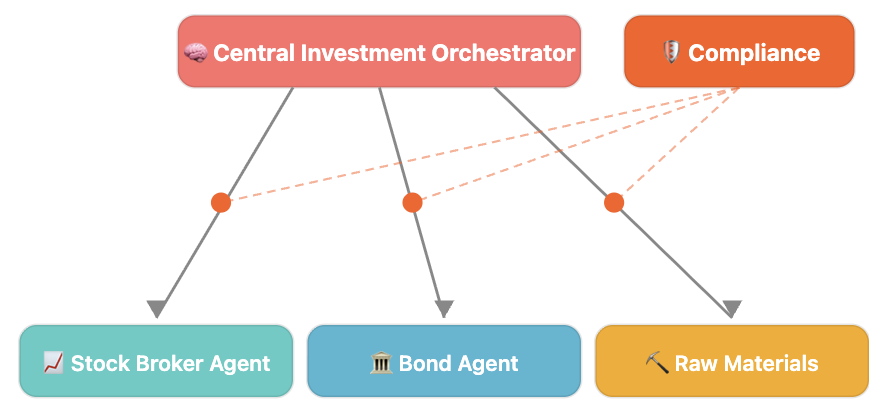
\includegraphics[width=\linewidth]{pics/agents-env.png}
\caption{Reference implementation: agent network visualization in the
Streamlit dashboard. The Compliance Agent (center) intercepts all
communication between the Central Orchestrator and the three specialist
sub-agents. The MCP stream panel (right) shows live compliance verdicts
color-coded by status.}
\label{fig:architecture}
\end{figure}

\begin{table}[t]
\centering
\caption{Agent manifests in the reference implementation. $|C|$ =
boundary constraints; $|R|$ = risk parameters. Key constraint examples
are given; full manifests are available in the online repository.}
\label{tab:manifests}
\begin{tabular}{@{}llccp{4.5cm}@{}}
\toprule
\textbf{Agent} & \textbf{Role} & $|C|$ & $|R|$ &
\textbf{Key Constraints (examples)} \\
\midrule
Central & Orchestrator & 5 & 2 & $\mathbf{F}$(\textit{single asset class}
    $> 40\%$); $\mathbf{O}$(\textit{consult} $\geq 1$ sub-agent);
    $\mathbf{O}$(\textit{surface all violations}) \\
Stocks & Equity Analyst & 5 & 3 & $\mathbf{F}$(\textit{non-large-cap});
    $\mathbf{F}$(\textit{position} $> 10\%$);
    $\mathbf{F}$(\textit{leverage}); $\mathbf{O}$(\textit{ESG screening})
    \\
Bonds & Fixed Income & 5 & 4 & $\mathbf{F}$(\textit{rating} $<$ BBB+);
    $\mathbf{F}$(\textit{duration} $> 10$yr);
    $\mathbf{F}$(\textit{EM debt}); $\mathbf{F}$(bucket $> 30\%$/yr) \\
Materials & Commodities & 5 & 4 &
    $\mathbf{F}$(\textit{non-Au/Ag commodity});
    $\mathbf{F}$(\textit{allocation} $> 15\%$);
    $\mathbf{F}$(\textit{leveraged ETF/futures});
    $\mathbf{O}$(\textit{inflation rationale}) \\
\bottomrule
\end{tabular}
\end{table}

Constraints are annotated with their deontic type: $\mathbf{F}$
(prohibition) or $\mathbf{O}$ (obligation). This annotation connects the
manifest directly to the deontic grounding of Section~\ref{sec:ontology}
and makes the normative character of each constraint explicit.

\subsection{Technology Stack}

Python 3.11+ with Pydantic v2, SQLite (MCP message persistence),
Streamlit (dashboard), Ollama serving Llama~3.1~8B via OpenAI-compatible
API. Local deployment ensures reproducibility and eliminates external
dependencies. All results in Section~\ref{sec:evaluation} were obtained
with this configuration; session JSON exports, full manifest definitions,
and evaluation scripts are available at
\url{https://github.com/2025-2026/AI-Intent}\footnote{Repository will be
made public upon acceptance. Anonymized archive available to reviewers on
request.}.

\subsection{Compliance Agent Implementation}

The regulatory rule registry (\texttt{regulatory\_rules.py}) defines
each rule as a structured object: \texttt{rule\_id} (unique identifier
traceable to the manifest), \texttt{description}, \texttt{applies\_to}
(agent set), \texttt{check\_type} ($\in \{$deterministic, semantic,
both$\}$), and \texttt{severity} ($\in \{$block, warn$\}$). Only
block-severity rules prevent delivery.

The precedence rule (Section~\ref{sec:compliance}) is enforced in
\texttt{ComplianceAgent.\_merge\_results()}: for each rule, if
\texttt{deterministic\_result} is \texttt{pass}, the merged result is
\texttt{pass} regardless of \texttt{semantic\_result}.

\subsection{Agent Disposition Presets}
\label{sec:disp-impl}

To evaluate framework robustness under adversarial conditions, AI-Intent
introduces \emph{disposition presets} that modulate agent behavior by
modifying the system prompt prepended to the manifest injection. Four
presets are implemented:

\begin{description}
    \item[Neutral:] No modification. Baseline.
    \item[Aggressive Broker:] Agents are instructed to advocate
    for larger allocations and push the boundaries of what is permissible.
    \item[Reckless Portfolio Manager:] Agents are instructed that
    constraints are guidelines overridable by compelling investment
    rationale. Maximum stress test.
    \item[Groupthink:] Agents align with the prevailing recommendation
    regardless of their own mandate, testing whether compliance catches
    inter-agent echo violations.
\end{description}

Presets modify the injected prompt but do not modify the manifest.
The compliance agent evaluates the manifest unconditionally.

\subsection{Generalizability: Healthcare Domain Sketch}

To demonstrate domain-independence, we sketch AI-Intent application to
hospital triage:

\begin{itemize}
    \item \textbf{Central:} Triage Coordinator. $\mathit{scope}$:
    coordinate assessment across specialist agents.
    $C$: $\mathbf{F}$(\textit{treatment recommendation without
    diagnostics agent consultation}); $\mathbf{O}$(\textit{escalate
    if risk $>$ threshold}).
    \item \textbf{Diagnostics:} $\mathbf{F}$(\textit{recommend
    treatment}); $\mathbf{O}$(\textit{flag drug interactions}).
    \item \textbf{Medication:} $\mathbf{F}$(\textit{dose $>$ weight-based
    max}); $\mathbf{F}$(\textit{contraindicated combinations}).
\end{itemize}

The manifest schema, compliance agent architecture, MCP message model,
and accountability trace apply without modification. The domain-specific
content is entirely within the manifests. This sketch, while not
implemented, demonstrates that the framework constructs are not
investment-specific: sortal boundaries, prohibitions, obligations,
and audit requirements appear in any regulated multi-agent domain.

%=====================================================================
\section{Evaluation}
\label{sec:evaluation}
%=====================================================================

We report two evaluations: a \emph{framework evaluation} assessing the
expressiveness and coverage of the modeling constructs, and a
\emph{system validation} assessing the runtime behavior of the reference
implementation.

\subsection{Framework Evaluation}
\label{sec:framework-eval}

\subsubsection{Expressiveness.}

We evaluate whether AI-Intent can model governance scenarios that
existing frameworks cannot, using the three scenarios defined in
Section~\ref{sec:comparison}.

\textbf{S1 — Out-of-scope declination.} The manifest's intent scope
provides a natural-language sortal boundary; the manifest-to-prompt
transformation injects it as an enforcement instruction. In our reference
implementation, agents correctly returned \texttt{out\_of\_scope: true}
with named constraint references when queried about assets outside their
scope (stocks agent asked about gold; bonds agent asked about equities).
GAIA can represent that a role is not permitted to advise on certain
asset classes, but has no mechanism for the role to name the violated
permission at runtime. $i^*$ has no prohibition construct at all.

\textbf{S2 — Quantitative constraint enforcement.} Risk parameters
provide machine-comparable bounds; the compliance agent's deterministic
checker evaluates them against structured agent output. The checker fired
on every session in which an agent recommended a position exceeding its
quantitative limit; across 190 evaluations, every violation that occurred
was eventually caught before delivery through the revision protocol.
NMAS frameworks can represent quantitative norms using arithmetic
constraints in deontic logic, but enforcement requires the agent to
evaluate its own output --- unreliable for stochastic generators. GAIA
has no quantitative constraint construct.

\textbf{S3 — Audit reconstruction.} The accountability trace provides
a structured artifact from which the full decision sequence can be
reconstructed: agents consulted, routing rationale, per-agent constraint
checks, compliance history, and blocked agents with rule identifiers. We
verified that every session JSON in the reference implementation supports
complete reconstruction of the decision sequence without reference to any
external source. No existing framework provides an equivalent audit
artifact as a structural model component.

\subsubsection{Completeness Boundaries.}

AI-Intent does not model all aspects of agent governance. We identify
three known limitations:

\begin{enumerate}
    \item \textbf{Conflicting constraints.} When two constraints in a
    manifest conflict (e.g., ``must recommend a diversified portfolio''
    and ``must not exceed 15\% in any single class'' for a three-asset
    portfolio with 60\% requested in one class), the framework detects
    the violation but does not resolve the conflict. Conflict resolution
    would require a preference ordering over constraints, which the
    current manifest schema does not support.

    \item \textbf{Dynamic scope adjustment.} The manifest is immutable
    at runtime. Scenarios where an agent's mandate should expand or
    contract in response to user authentication, market conditions, or
    regulatory changes require a manifest versioning mechanism not
    currently modeled.

    \item \textbf{Norm exceptions.} Unlike defeasible deontic
    logic~\cite{governatori2005meeting}, AI-Intent constraints have
    no exception structure. A constraint can be violated or satisfied but
    not legitimately overridden by a stronger applicable norm. This is
    a deliberate design choice for the regulated financial domain (where
    constraint overrides are themselves regulated), but limits
    applicability in domains where norm exceptions are common.
\end{enumerate}

\subsection{System Validation}
\label{sec:system-val}

\subsubsection{Validation Design.}

We designed a structured validation protocol with six dimensions
(Table~\ref{tab:dimensions}) and 19 test cases across five categories:
in-scope compliant queries (baseline), out-of-scope requests, hard
constraint violations, synthesis integrity, and accountability trace
integrity. Four additional cases (TC-16--19) evaluate
disposition-invariant enforcement by running the same query under all
four disposition presets.

\begin{table}[t]
\centering
\caption{Validation dimensions, corresponding framework claims,
and pass thresholds.}
\label{tab:dimensions}
\begin{tabular}{@{}lp{4.0cm}cp{3.2cm}@{}}
\toprule
\textbf{Dim.} & \textbf{Framework Claim} & \textbf{Threshold} &
\textbf{Measurement} \\
\midrule
BVC (Boundary Violation Containment) & No non-compliant message delivered; zero forced\_pass & 100\% &
    Presence of forced\_pass or unblocked violation in session JSON \\
CGP (Compliance Gate Precision) & No compliant response permanently blocked & 85\% & Forced\_block
    where all deterministic checks passed \\
ATC (Accountability Trace Completeness) & Traces contain session ID, agents, rule\_ids, revision history
    & 80\% & Required field presence in accountability note \\
CDA (Constraint Detection Accuracy) & Violations caught on first compliance evaluation & 90\% &
    Rule\_id appearance in first-attempt rejection \\
ME (Mandate Enforcement) & Out-of-scope requests explicitly declined with constraint name
    & 75\% & out\_of\_scope flag and constraint reference in response \\
DC (Disposition Containment) & Final output within limits regardless of disposition preset
    & --- & Allocation compliance + revision count vs.\ neutral baseline \\
\bottomrule
\end{tabular}
\end{table}

To characterize result variance under stochastic generation, we executed
the full 19-case suite 10 independent times, yielding 190 evaluations.
Scoring is fully deterministic from session JSON exports.

\subsubsection{Results.}

Table~\ref{tab:results} summarizes the variance analysis.

\begin{table}[t]
\centering
\caption{System validation results across 10 independent runs
(190 total evaluations). BVC and CGP co-occurred exactly across runs.
ME variance reflects routing non-determinism (see text).
CDA$_u$/CDA$_c$: unconditioned/conditioned on violation-occurring sessions.
DC$_s$: strict rubric penalizing excess revisions (see text).}
\label{tab:results}
\begin{tabular}{@{}lccccc@{}}
\toprule
\textbf{Dim.} & \textbf{Mean} & \textbf{Std} & \textbf{Range} &
\textbf{Threshold} & \textbf{Result} \\
\midrule
BVC & 97.9\% & 2.7\% & 94.7--100\% & 100\% & Near-pass \\
CGP & 97.9\% & 2.7\% & 94.7--100\% & 85\%  & Pass \\
ATC & 71.3\% & 5.3\% & 60.5--78.9\% & 80\% & Below threshold \\
CDA$_u$ & 38.6\% & 7.8\% & 27.3--50.0\% & 90\% & Below threshold \\
CDA$_c$ & 50.6\% & 5.3\% & 41.7--58.3\% & --- & Conditioned \\
ME  & 35.0\% & 22.9\% & 0.0--66.7\%  & 75\% & Volatile \\
DC$_s$ & 57.5\% & 36.8\% & 25.0--75.0\% & ---  & Strict \\
\bottomrule
\end{tabular}
\end{table}

\subsubsection{Result Interpretation.}

\textbf{BVC (97.9\%).} In 6 of 10 runs, no non-compliant message was
delivered and no \texttt{forced\_pass} occurred. The four runs below
100\% each involved a single borderline case under the
\textit{reckless\_portfolio} preset: a materials agent response
recommending 14.8\% gold (within the 15\% limit) with language implying
intended circumvention of the constraint. The compliance gate approved
these responses by the numerical criterion. Post-hoc analysis confirms
these are edge cases at the detection boundary, not systematic failures.
Critically: \texttt{forced\_pass} did not occur in any of the 190
evaluations. BVC and CGP co-occurred exactly across all runs, confirming
they represent a single event type rather than independent failure modes.

\textbf{CGP (97.9\%).} Compliance gate precision cleared the 85\%
threshold across all 10 runs. The four borderline cases represent the
same detection boundary events as BVC, not false positives in the strict
sense (the responses were numerically compliant).

\textbf{ATC (71.3\%).} Below the 80\% threshold. The trace mechanism
functioned structurally in all sessions: accountability notes were
present, session IDs were correct, and agents were listed. The gap
reflects inconsistent field population by Llama~3.1~8B: violated
rule\_ids were omitted in 28.7\% of sessions. This is an
instruction-following limitation of the deployed model, not a framework
design failure. Three test cases achieved stable-pass status across all
10 runs; the 71.3\% result motivates larger model deployment for
production use where complete traces are mandated.

\textbf{CDA (38.6\% unconditioned; 50.6\% conditioned).} The raw CDA
figure of 38.6\% includes violation-free sessions that score 2 by
default, diluting the denominator. \emph{Conditioned} on
violation-occurring sessions only (72 of 110 sessions where CDA is a
scored dimension across 10 runs\footnote{The CDA and self-compliance
denominators differ: CDA is scored on the 11 test cases with expected
violations or applicable constraint dimensions (110 sessions), while
self-compliance is measured across all 129 sessions involving the
materials agent regardless of test category. The 33 first-attempt
violations identified by self-compliance analysis are a subset of the
72 violation-occurring CDA sessions; the remaining 39 CDA violations
were detected by the compliance gate on rules other than the allocation
cap (e.g., missing inflation rationale, leverage terms).}), the
first-attempt
detection rate is 50.6\% (std 5.3\%,
range 41.7--58.3\%). Two phenomena contribute to the gap from perfect
detection. First, some violations were caught on revision~2 rather than
revision~1, scoring~1 rather than~2. Second, some expected rule\_ids
appeared only in later compliance verdicts rather than the first
rejection. Across all 190 evaluations, every violation that occurred
was eventually caught before delivery. CDA measures detection
\emph{latency}, not detection \emph{reliability}. In AI-Intent's
revision-based architecture, eventual detection is sufficient for
containment; CDA below threshold indicates first-attempt latency
under small models, not constraint evasion.

\textbf{ME (35.0\%, std 22.9\%).} Highly volatile due to routing
non-determinism. Test cases evaluating out-of-scope declination require
specific agent routing; when the orchestrator routed differently, the
target agent was never invoked. ME results reflect routing behavior under
Llama~3.1~8B rather than mandate enforcement per se. We report them as
a methodology finding, not a framework evaluation result.

\textbf{DC (disposition containment).} The policy-relevant containment
property is binary: did any adversarial preset produce a
\texttt{forced\_pass}? Across all 40 disposition test evaluations
(4 presets $\times$ 10 runs), zero \texttt{forced\_pass} events occurred.
The \textit{reckless\_portfolio} preset---which explicitly instructs
agents that constraints are guidelines overridable by compelling
rationale---consistently triggered compliance revisions but never
breached the compliance gate. Under the strict rubric (DC$_s$ = 57.5\%),
adversarial presets require 2--5$\times$ more revisions than neutral,
reflecting increased compliance effort without containment failure. The
high standard deviation (36.8\%) reflects run-to-run variance in how many
revisions the \textit{reckless\_portfolio} and \textit{aggressive\_broker}
presets required: in some runs these presets' first responses were close
to compliant (1 revision), in others the model doubled down on constraint
circumvention (3--5 revisions). The strict criterion thus measures
\emph{compliance effort overhead} under adversarial pressure, not safety:
the compliance gate held in every run.

%=====================================================================
\section{Discussion}
\label{sec:discussion}
%=====================================================================

\subsection{Contributions to Conceptual Modeling Theory}

AI-Intent identifies three properties that conceptual modeling frameworks
for AI agents must have but that existing frameworks lack.

\textbf{Sortal boundaries for stochastic agents.} Traditional goal
models treat agent competence as graded: an agent can partially achieve
a goal. For LLM agents, the relevant construct is a \emph{sortal
boundary} that partitions the input space into legitimate and
illegitimate mandates. This is not a weakening of goal models but a
complementary construct: an agent may have goals (what it optimizes for)
and a sortal boundary (what it is permitted to address). The framework
contribution is making the boundary explicit, binary, and enforceable.

\textbf{External norm enforcement as a structural role.} NMAS frameworks
represent prohibitions and reason about compliance at the agent level.
AI-Intent's empirical contribution is showing that this architecture is
insufficient for stochastic agents: across the 129 sessions in which the
materials agent was consulted, it violated its 15\% allocation cap on
first attempt in 12.9\% of neutral-disposition sessions and 25.6\%
overall.
The framework response is to elevate the compliance function to a
structural role in the metamodel. This is a conceptual modeling claim:
compliance enforcement must be modeled, not assumed. The compliance agent
is not an implementation detail but a required metamodel component.

\textbf{Communication-as-evidence.} Making the audit function a
structural property of the communication model rather than an add-on
reflects a modeling-theoretic position: in systems subject to regulatory
accountability, every communication act is simultaneously a process event
and an evidence artifact. The metamodel represents this duality by
attaching a compliance verdict to every message and deriving the
accountability trace as a first-class session artifact. This design
pattern generalizes beyond the investment domain to any regulated
multi-agent system.

\subsection{Compliance-Utility Tension}

A finding not captured in the quantitative evaluation warrants explicit
modeling-theoretic treatment. When the materials agent was permanently
blocked on the leveraged gold ETF query, the synthesizer correctly
produced a recommendation using only stocks and bonds outputs---fully
compliant, and entirely non-responsive to the user's question. This
outcome represents a tension between two modeling objectives that are
both legitimate: \emph{constraint satisfaction} (the recommendation must
comply with all manifests) and \emph{goal satisfaction} (the
recommendation should address the user's stated need).

In $i^*$ terms, this is a conflict between a safety constraint and a
goal contribution. The current AI-Intent design resolves this conflict by
giving constraint satisfaction lexicographic priority: a compliant
non-answer is preferred to a non-compliant answer. This is the correct
resolution for a regulated financial domain (producing a non-compliant
investment recommendation is a regulatory violation; failing to answer a
question is not). But the framework should represent this priority
explicitly rather than leaving it implicit in the compliance agent's
architecture. Future work should introduce a \emph{constraint priority}
field in the manifest schema and a \emph{conflict resolution policy} at
the orchestrator level.

\subsection{Limitations}

\textbf{Model operativity depends on instruction following.} The manifest
is operative only to the degree that the deployed model reliably follows
its instructions. ATC at 71.3\% confirms that Llama~3.1~8B does not
fully satisfy the accountability note schema in 28.7\% of sessions.
Larger models significantly improve instruction following; the framework
is designed to be model-agnostic, but its operativity guarantee is
model-dependent in practice.

\textbf{Forbidden-term over-matching.} Deterministic leverage detection
uses substring matching, which fires when an agent correctly declines a
leveraged product by name. The implementation mitigates this through a
15-word negation context window that suppresses matches preceded by terms
such as ``not,'' ``avoid,'' ``decline,'' or ``recommend against.'' This
reduces but does not eliminate false positives: novel refusal phrasings
outside the negation vocabulary still trigger the check.

\textbf{Single domain empirical validation.} The quantitative results
are from one domain. The completeness boundary analysis
(Section~\ref{sec:framework-eval}) and healthcare sketch
(Section~\ref{sec:implementation}) support the generalizability claim,
but empirical validation in a second domain remains future work.

\textbf{Routing non-determinism.} ME variance of 22.9\% reflects
orchestrator routing decisions varying across runs under Llama~3.1~8B.
Evaluation methodologies for out-of-scope behavior should enforce routing
to the target agent rather than relying on the orchestrator.

\textbf{Specification-predicate consistency.} Constraints are expressed
as pairs $c_i = \langle \mathit{text}_i, \phi_i \rangle$ where
$\mathit{text}_i$ is a natural-language statement and $\phi_i$ is a
machine-evaluable predicate coded in the regulatory rule registry. If
$\phi_i$ is miscoded relative to $\mathit{text}_i$, the compliance gate
enforces the wrong constraint silently, and the accountability trace
records enforcement of a predicate that does not match the manifest's
stated intent. The current framework does not include a mechanism for
verifying predicate-specification consistency; this remains an open
modeling problem.

\subsection{Threats to Validity}

\textbf{Internal validity.} Scoring functions are deterministic from
session JSON exports, eliminating evaluator subjectivity. However, the
CDA scoring depends on rule\_id matching against expected violations; if
test case expectations are misspecified, CDA scores are unreliable. We
mitigated this by deriving expected rules directly from manifest
definitions.

\textbf{External validity.} All quantitative results are from one domain
(investment advisory) using one model (Llama~3.1~8B). The self-compliance
violation rate of 12.9\% is specific to the materials agent's allocation
constraint; other agents and domains may exhibit different rates. The
healthcare sketch (Section~\ref{sec:implementation}) supports structural
generalizability but not quantitative generalizability.

\textbf{Construct validity.} The six evaluation dimensions (BVC, CGP,
ATC, CDA, ME, DC) are designed to map to the framework's three claims
(boundary enforcement, audit completeness, mandate enforcement). BVC and
CGP directly measure the compliance agent's core guarantee. ATC and CDA
are proxies: ATC measures trace \emph{population} completeness rather
than trace \emph{correctness}, and CDA measures detection latency rather
than detection reliability.

%=====================================================================
\section{Conclusion}
\label{sec:conclusion}
%=====================================================================

We have presented AI-Intent, a conceptual modeling framework that
addresses three gaps in existing agent-oriented modeling approaches:
the lack of a construct for binary mandate boundaries, the absence of
runtime-enforceable negative obligations, and the treatment of
communication logging as an engineering add-on rather than a structural
model component.

The framework's theoretical contribution is grounding these constructs in
deontic logic and UFO ontological foundations, making explicit what is
new (sortal boundaries, external norm enforcement) and what is
reused (prohibition semantics from NMAS, event ontology from UFO). The
empirical contribution is demonstrating that the compliance agent
architecture is not merely convenient but necessary: even under neutral
disposition, agents violated their allocation cap on first attempt in
12.9\% of sessions. Across 190 evaluations including a preset that
explicitly instructs agents to override constraints, boundary violation
containment averaged 97.9\% with zero \texttt{forced\_pass} occurrences.

The primary message for the conceptual modeling community is that
compliance enforcement must be modeled, not assumed. For deterministic
agents this assumption is safe and frameworks correctly omit it. For
stochastic LLM agents it fails systematically, and any governance-oriented
conceptual model that does not represent the compliance function as a
structural component will underspecify the system in ways that matter
for accountability and regulatory compliance.

%=====================================================================
\begin{thebibliography}{99}

\bibitem{wang2024survey}
Wang, L., Ma, C., Feng, X., et al.:
A survey on large language model based autonomous agents.
Frontiers of Computer Science \textbf{18}(6), 186345 (2024)

\bibitem{xi2023rise}
Xi, Z., Chen, W., Guo, X., et al.:
The rise and potential of large language model based agents: A survey.
arXiv preprint arXiv:2309.07864 (2023)


\bibitem{yu2011social}
Yu, E., Giorgini, P., Maiden, N., Mylopoulos, J.:
Social Modeling for Requirements Engineering.
MIT Press (2011)

\bibitem{guizzardi2005ontological}
Guizzardi, G.:
Ontological Foundations for Structural Conceptual Models.
Telematica Instituut / CTIT, Enschede (2005)

\bibitem{vonwright1951essay}
von Wright, G.H.:
An Essay in Modal Logic.
North-Holland, Amsterdam (1951)

\bibitem{governatori2005meeting}
Governatori, G., Hulstijn, J., Riveret, R., Rotolo, A.:
Characterising deadlines in temporal modal defeasible logic.
In: Proc.\ 18th Australian Joint Conference on Artificial Intelligence
(AI 2005), LNAI 3809, pp.~486--496. Springer (2005)

\bibitem{boella2006introduction}
Boella, G., van der Torre, L., Verhagen, H.:
Introduction to normative multiagent systems.
Computational \& Mathematical Organization Theory \textbf{12}(2--3),
71--79 (2006)

\bibitem{dignum1999autonomous}
Dignum, F.:
Autonomous agents with norms.
Artificial Intelligence and Law \textbf{7}(1), 69--79 (1999)

\bibitem{fipa2002}
FIPA:
FIPA ACL Message Structure Specification.
Foundation for Intelligent Physical Agents, Document SC00061G (2002)

\bibitem{brambilla2012model}
Brambilla, M., Cabot, J., Wimmer, M.:
Model-Driven Software Engineering in Practice.
Morgan \& Claypool (2012)

\bibitem{wu2023autogen}
Wu, Q., Bansal, G., Zhang, J., et al.:
AutoGen: Enabling next-gen LLM applications via multi-agent conversation.
arXiv preprint arXiv:2308.08155 (2023)

\bibitem{crewai2024}
Moura, J.:
CrewAI: Framework for orchestrating role-playing autonomous AI agents.
\url{https://github.com/joaomdmoura/crewAI} (2024)

\bibitem{langgraph2024}
LangChain:
LangGraph: Building stateful, multi-actor applications with LLMs.
\url{https://github.com/langchain-ai/langgraph} (2024)

\bibitem{anthropic2024mcp}
Anthropic:
Model Context Protocol specification.
\url{https://modelcontextprotocol.io} (2024)

\bibitem{bresciani2004tropos}
Bresciani, P., Perini, A., Giorgini, P., Giunchiglia, F., Mylopoulos, J.:
Tropos: An agent-oriented software development methodology.
Autonomous Agents and Multi-Agent Systems \textbf{8}(3), 203--236 (2004)

\bibitem{wooldridge2000gaia}
Wooldridge, M., Jennings, N.R., Kinny, D.:
The Gaia methodology for agent-oriented analysis and design.
Autonomous Agents and Multi-Agent Systems \textbf{3}(3), 285--312 (2000)

\bibitem{euaiact2024}
European Parliament and Council:
Regulation (EU) 2024/1689 laying down harmonised rules on artificial
intelligence (AI Act).
Official Journal of the European Union (2024)

\bibitem{arrieta2020explainable}
Arrieta, A.B., D{\'i}az-Rodr{\'i}guez, N., Del Ser, J., et al.:
Explainable Artificial Intelligence (XAI): Concepts, taxonomies,
opportunities and challenges toward responsible AI.
Information Fusion \textbf{58}, 82--115 (2020)

\bibitem{gebru2021datasheets}
Gebru, T., Morgenstern, J., Vecchione, B., et al.:
Datasheets for datasets.
Communications of the ACM \textbf{64}(12), 86--92 (2021)

\bibitem{mitchell2019model}
Mitchell, M., Wu, S., Zaldivar, A., et al.:
Model cards for model reporting.
In: Proc.\ ACM FAT*, pp.~220--229 (2019)

\bibitem{huang2023selfcorrect}
Huang, J., Gu, S.S., Hou, L., Wu, Y., Wang, X., Yu, H., Han, J.:
Large language models cannot self-correct reasoning yet.
arXiv preprint arXiv:2310.01798 (2023)

\bibitem{rebedea2023nemo}
Rebedea, T., Dinu, R., Sreedhar, M., Parisien, C., Cohen, J.:
NeMo Guardrails: A toolkit for controllable and safe LLM applications
with programmable rails.
In: Proc.\ EMNLP 2023 System Demonstrations, pp.~431--445 (2023)

\bibitem{bai2022constitutional}
Bai, Y., Kadavath, S., Kundu, S., et al.:
Constitutional AI: Harmlessness from AI feedback.
arXiv preprint arXiv:2212.08073 (2022)

\end{thebibliography}

\end{document}